%\documentclass[sigconf]{acmart} 
\documentclass[10pt, sigconf, format=acmsmall, screen=true, review=false]{acmart} 
\usepackage{amsmath}
\usepackage{amsfonts}
\usepackage{amssymb}
\usepackage{hyperref}
\usepackage{pdfpages} % http://mirror.unl.edu/ctan/macros/latex/contrib/pdfpages/pdfpages.pdf
\usepackage{booktabs} 
\usepackage{url}
% By default the URLs are put in typewriter type in the body and the
% bibliography of the document when using the \url command.  If you are
% using many long URLs you may want to uncomment the next line so they
% are typeset a little smaller.
%\renewcommand{\UrlFont}{\small\tt}

\usepackage[utf8]{inputenc}
\usepackage{graphicx}
%\usepackage[colorinlistoftodos]{todonotes} % handig voor commentaar: gebruik \todo{}, zie ftp://ftp.fu-berlin.de/tex/CTAN/macros/latex/contrib/todonotes/todonotes.pdf
\usepackage{listings}
 
\usepackage{tcolorbox}
\usepackage{float}
\usepackage{caption}
\usepackage{subcaption}

% For todos, notes from other authors, etc.
\usepackage[show]{chato-notes}
%Turn off footing
\settopmatter{printacmref=false}
\fancyfoot{}
%Turn off page numbering
\pagestyle{empty}

\usepackage{multirow}

\newcommand{\shorttitle}{Job Recommender System for Welfare Beneficiaries} % Put your short title here

\begin{document}

%\input{titlepage}
%\documentclass[]{article}
%\usepackage{lmodern}
%%\usepackage{fontspec}
%\usepackage{amssymb,amsmath}
%\usepackage{ifxetex,ifluatex}
%\usepackage{fixltx2e} % provides \textsubscript
%\ifnum 0\ifxetex 1\fi\ifluatex 1\fi=0 % if pdftex
%  \usepackage[T1]{fontenc}
%  \usepackage[utf8]{inputenc}
%\else % if luatex or xelatex
%  \ifxetex
%    \usepackage{mathspec}
%    \usepackage{xltxtra,xunicode}
%  \else
%    \usepackage{fontspec}
%  \fi
%  \defaultfontfeatures{Mapping=tex-text,Scale=MatchLowercase}
%  \newcommand{\euro}{€}
%\fi
%% use upquote if available, for straight quotes in verbatim environments
%\IfFileExists{upquote.sty}{\usepackage{upquote}}{}
%% use microtype if available
%\IfFileExists{microtype.sty}{%
%\usepackage{microtype}
%\UseMicrotypeSet[protrusion]{basicmath} % disable protrusion for tt fonts
%}{}
%\usepackage{graphicx}
%\makeatletter
%\def\maxwidth{\ifdim\Gin@nat@width>\linewidth\linewidth\else\Gin@nat@width\fi}
%\def\maxheight{\ifdim\Gin@nat@height>\textheight\textheight\else\Gin@nat@height\fi}
%\makeatother
%% Scale images if necessary, so that they will not overflow the page
%% margins by default, and it is still possible to overwrite the defaults
%% using explicit options in \includegraphics[width, height, ...]{}
%\setkeys{Gin}{width=\maxwidth,height=\maxheight,keepaspectratio}
%\ifxetex
%  \usepackage[setpagesize=false, % page size defined by xetex
%              unicode=false, % unicode breaks when used with xetex
%              xetex]{hyperref}
%\else
%  \usepackage[unicode=true]{hyperref}
%\fi
%\hypersetup{breaklinks=true,
%            bookmarks=true,
%            pdfauthor={},
%            pdftitle={},
%            colorlinks=true,
%            citecolor=blue,
%            urlcolor=blue,
%            linkcolor=magenta,
%            pdfborder={0 0 0}}
%\urlstyle{same}  % don't use monospace font for urls
%\setlength{\parindent}{0pt}
%\setlength{\parskip}{6pt plus 2pt minus 1pt}
%\setlength{\emergencystretch}{3em}  % prevent overfull lines
%\setcounter{secnumdepth}{0}
%
%\date{}
%
%\begin{document}


\begin{titlepage}


\begin{center}
 
\textsc{\Large   Job Recommender System for Welfare Beneficiaries}

\bigskip

\textsc{\large
submitted in partial fulfillment for the degree of master of science\\
%
\bigskip
Jasper Adema\\
%
11879394\\
%
\bigskip
master information studies\\
%
data science \\
%
faculty of science\\
%
university of amsterdam\\
%
\bigskip
2019-07-19
}

\end{center}
 

\vfill

% In case of an internal project, remove External Supervisor or if you had two internal supervisors, change the header into 
%  & First Supervisor & Second Supervisor  \\
\begin{center}
\begin{tabular}{|l||ll|}
\hline
 & \textbf{Internal  Supervisor} & \textbf{External   Supervisor}  \\   
 \hline
\textbf{Title, Name} & H.R. Oosterhuis &  L. van Oirschot\\
\textbf{Affiliation} &University of Amsterdam & Municipality of Amsterdam\\ 
\textbf{Email} & harrieoosterhuis@uva.nl& l.van.oirschot@amsterdam.nl\\
\hline
\end{tabular}
\end{center}



%% If you have a third supervisor use this table instead
%\begin{center}
%\begin{tabular}{|l||lll|}
%\hline
% & \textbf{External   Supervisor} & \textbf{External   Supervisor} & \textbf{3$^{\mathrm{rd}}$ supervisor} \\
% \hline
%\textbf{Title, Name} & Dr Maarten Marx& & \\
%\textbf{Affiliation} &UvA, FNWI, IvI & & \\ 
%\textbf{Email} & maartenmarx@uva.nl& &  .\\
%\hline
%\end{tabular}
%\end{center}

\bigskip

% logos
\begin{center}
\mbox{\includegraphics[width=.2\paperwidth]{TitlePages/logos/logo-uva.png} 
\includegraphics[width=.2\paperwidth]{TitlePages/logos/ads.png}

\includegraphics[width=.2\paperwidth]{TitlePages/logos/Selection_272.png}
 % replace by the logo of your internship company or add
}
\end{center}
\end{titlepage}

%
%\newpage
%
%\end{document}
  % or use another template

\pagebreak

\pagebreak
%Change the font size to a smaller type
% \small
\footnotesize
% \scriptsize
% \tiny


%Main body of the document
%Set two column format for document
\twocolumn

%Abstract
\section*{Abstract}
In this paper a feasibility study of a Content-Based Job Recommender System (JRS) for welfare beneficiaries is described.
It is found that the Neural Network is the best model for learning to predict a job match. 
However, this model does not translate into a good top-\textit{n} rank recommender. 
Methods for dealing with label sparsity and practical approaches to better the performance proved to be ineffective. 
The mediocre results are likely caused by the fact that the data is biased and noisy, as well as that there is not enough data available.
Therefore the outcomes of this research highlight the importance of the quality and quantity of the data for the success of a JRS.
Given the used data a JRS is currently not feasible, however if measures are taken to improve the data it can be in the future.

\section*{Keywords}
Recommender Systems, Job Recommender System, Welfare Benefits, Machine Learning, Clustering, Deep Learning

% Here you input all your sections in separate files
\section{Introduction}
\label{sec:intro}

% \mynote[author=Harrie]{Voorbeeld van commentaar vanuit Harrie.}

%body
% \todo{Motivatie voor job recommendation}
% \todo{Motivatie voor jouw werk (toevoeging/contributie)}
% \todo{uitlijning van wat er gaat komen}
% \todo{RQ}
% \todo{specificatie van jouw project met de gemeente Amsterdam}


%Motivatie voor job recommendations
The digitalization of our society has made information more easily accessible than ever before.
When, for example, buying a product or choosing a movie to watch people are presented with myriad of choices. 
However more choices do not always equal to better choices, this paradox of choice especially occurs when people are overloaded with information \cite{schwartz2004paradox}. 
Recommender Systems (RS) are software tools and techniques designed to aid people in making choices by selecting and presenting items to them that could be of their interest.

RSs are applied in many different domains \cite{aggarwal2016recommender}, famous examples of companies using RSs are Amazon (products and services), Netflix (movies), Spotify (music), Facebook (content) and LinkedIn (jobs).
For matching job seekers with job vacancies RSs are a useful tool to find the best job openings, or visa versa for recruiters to find the best candidates for a job.
The job recommendation problem is essentially different from other traditional recommendation problems such recommending products or movies to users.
The main difference is that a same product or movie can potentially be recommended to thousands of consumers, while a job vacancy is usually posted with the goal to hire one or only a couple of employees.

%Motivatie voor jouw werk (toevoeging/contributie)
Today the application of Job Recommender Systems (JRS) is mostly restricted to online platforms. 
LinkedIn for example claims that its JRS is crucial in helping to achieve its company goals \cite{kenthapadi2017personalized}.
While online job boards and professional social networks such as Indeed and Linkedin can aid most people in finding a job, they are not always suitable for people at the lower end of the labor market.
A group of people who are often positioned at the lower end of the labor market are welfare beneficiaries. 
The composition of the group of welfare beneficiaries is characterized by a strong representation of immigrants, older people, people with low education, and people who suffer from mental or physical disabilities \cite{dodeweerd}.
Due to the special needs and characteristics of welfare beneficiaries a different and novel application of a RS is required. 
The goal of this type of JRS is, by taking into account the special needs and characteristics of welfare beneficiaries, to make better and more lasting matches between them and job openings.
Such a system would operate at the intersection of RSs, information retrieval, machine learning and statistical optimization. 

The research presented in this paper will focus on the job recommendation problem and its related machine learning challenges for the group of welfare beneficiaries in the city of Amsterdam. 

%Main Research Question
The paper aims to answer the following Research Question:
\begin{enumerate}
    \item \em Can a Content-Based Recommender System based on matching job openings to welfare beneficiaries be comparable to human customer managers? \label{rq:mrq}
\end{enumerate}{}

%Sub Research Questions
The subquestions we answer are:
\begin{enumerate}\addtocounter{enumi}{1}
    \item Can clustering deal with label sparsity in job matching data? \label{rq:cold}
    \item Are there significant differences between models in predictive performance? \label{rq:model}
    \item Does a model trained for prediction of job matches translate to a good ranking-based recommender? \label{rq:ranking}
    \item Does feature selection and addressing class imbalance have a significant effect on the predictive performance? \label{rq:strategies}
\end{enumerate}

%uitlijning van wat er gaat komen
The paper is structured as follows. First, related previous studies are discussed (section \ref{sec:rel}). Next, the methodology and machine learning models are elaborated (section \ref{sec:meth}). This is followed by a description of the experimental setup (section \ref{sec:setup}). Hereafter the results are presented (section \ref{sec:rslts}). Then the outcomes and limitations of the research are discussed (section \ref{sec:disc}). After that the conclusions are drawn based on the findings (section \ref{sec:concl}). Finally, the future extensions of the research are explored (section \ref{sec:fut}).

%specificatie van jouw project met de gemeente Amsterdam
As part of the project “Optimalisatie Proces Begeleiden naar Werk en Participatie” the municipality of Amsterdam has supplied the data for this research. 
The aim of the this project is to reduce the number of welfare beneficiaries by getting them employed.
Creativity in applying novel technologies is conceived by the municipality to play an important role in achieving the objectives.
The learnings described in this paper can provide the city of Amsterdam with guidelines for the implementation of an intelligent and data driven system to match welfare beneficiaries with job opportunities. 




\section{Related Work}
\label{sec:rel}

%Introduction
This section provides an overview of the previous research done on Recommender Systems in general (\ref{sec:rs}), Job Recommender Systems (\ref{sec:jrs}), clustering and the cold-start problem (\ref{sec:ccs}), Content-Based models (\ref{sec:cbm}), and privacy by design (\ref{sec:pbd}).

%Recommender Systems
\subsection{Recommender Systems}
\label{sec:rs}
A Recommender System (RS) is a system that recommends items to users based on its transactional value \cite{aggarwal2016recommender}. With regard to this research, items are defined as job vacancies, the users as the welfare beneficiaries, and the transactional value as a fitting match between a welfare beneficiary and a job opening.

Within the domain of RSs there are many different types of RSs each with their own area of application and strengths and weaknesses.
A comprehensive taxonomy by Burk identifies five types of RSs: 1) Content-Based, 2) Collaborative Filtering, 3) Demographic, 4) Knowledge-Based, and 5) Hybrid Recommender Systems \cite{Burke2007HybridSystems}.
The characteristics of these types of RSs will be elaborated briefly.
With \textit{Content-Based} the system learns to recommend items that are similar to the ones the users have preferred in the past. 
The goal is to match the attributes of the users profile with the attributes of the items  \cite{aggarwal2016recommender}. 
\textit{Collaborative Filtering} in its most basic form generates recommendations for the users based on items that other similar users matched with in the past \cite{Schafer2007}.
A \textit{Demographic} system recommends items based on the demographic profile of the user \cite{Bobadilla2013RecommenderSurvey}.
At this time this is still a relatively unexplored area of RS research. \textit{Knowledge-Based} systems utilize domain knowledge about users to do the matching with particular item features to recommend items  \cite{aggarwal2016recommender}. 
Finally, \textit{Hybrid Recommender Systems} combine the earlier mentioned techniques and try to leverage the advantages of these particular systems and to mitigate their weaknesses  \cite{aggarwal2016recommender}.

In its most basic form a RS predicts the value over pairs of users and items to return the ones with the best utility scores.
Based on the literature RSs are thought to be a promising method for predicting job matches.

%Job Recommender Systems
\subsection{Job Recommender Systems}
\label{sec:jrs}
The previous section described RSs in general. 
In this part the literature of a specific type RS will be described: the Job Recommender System (JRS).
Traditional RSs can provide the same item (such a book, music or a movie) to thousands of different users.
The job recommendation problem is radically different because most job openings seek one or only a few employees to match with \cite{kenthapadi2017personalized}.

Most JRSs that operate today are proprietary, examples of companies who have developed a proprietary JRS are LinkedIn and Indeed.
According to studies conducted by Otaibi et al. and Zheng et al. the most commonly used  systems for Job recommendation are Collaborative Filtering, Content-Based, or a combination of both (Hybrid Recommender Systems) \cite{T.Al-Otaibi2012ASystems, Zheng2012JobSurvey}.
A study by Hong et al. (2013) investigates the implementation of four online JRSs and shows that all use a content-based recommender as its basis \cite{hong2013job}.
Kenthapadi et al. (2017) describe that LinkedIn has developed a hybrid JRS that uses content-based filtering as its basis \cite{kenthapadi2017personalized}.

JRSs are a special form of RS particular geared towards recommending jobs to users, and therefore applicable for the objective of our research. 

%Clustering and Cold-Start Problem
\subsection{Clustering and the Cold-Start Problem}
\label{sec:ccs}
RSs and especially JRSs are likely to suffer from the so-called cold-start problem, which is that items are rated only once or a few times by users.

According to Aggarwal et al. (2016) clustering is most often applied within RSs to solve the cold-start problem \cite{aggarwal2016recommender}.
The cold start problem is defined by Lika et al. (2014) as that the RS cannot recommend a user or item that is not yet rated \cite{lika2014facing}.
A study by Son (2016) which compares the various techniques of dealing with the cold-start problem for users, shows that clustering is often used to mitigate the cold-start problem \cite{son2016dealing}.

In 1979 Hartigan and Wong presented the K-means clustering algorithm \cite{hartigan1979algorithm}, and today it is the most used clustering algorithm in RSs \cite{aggarwal2016recommender}.
The K-means clustering algorithm tries to split a number of observations into clusters (\textit{K}) by assigning each observation to the cluster with the closest mean.
By reassigning the cluster centroids on each iteration the objective is to minimize a criterion known as the within-cluster sum-of-squares (also called inertia) \cite{mackay2003example}. 
K-means is less suitable for categorical data due to the way it calculates the distances between observations.
A variation on the K-means for categorical data is K-modes which uses modes instead of means to form clusters and tries to optimize a cost function \cite{huang1997clustering, huang1998extensions}.
The K-prototypes clustering algorithm which is also based on K-means can handle both numerical and categorical data at the same time \cite{huang1997clustering}.

Another less regular applied clustering algorithm within RS due its computational complexity is hierarchical clustering.
Whereas with the aforementioned K-means and K-modes clustering algorithms it is necessary to specify the desired number of clusters, the advantage of hierarchical clustering is that this is not required \cite{rokach2005clustering}.
However, the required computation time makes hierarchical clustering less suitable for medium and larger datasets. 

The cold-start problem is an issue associated with JRSs and clustering seems to be a promising method to tackle this problem.

%Content-Based Models
\subsection{Content-Based Models}
\label{sec:cbm}
There are various methods that can be used for a RS to learn to predict the utility of user and item pairs. 
In this part the literature regarding a method often applied for JRSs is described.

Pazzani and Billsus (2007) describe Content-Based Recommender Systems (CBRS) as systems that recommend an item to a user depending on the description of the item and a profile of the user’s preferences \cite{pazzani2007content}.
The core of a CBRS is the learning of user profiles to predict user interests in items by leveraging user feedback \cite{aggarwal2016content}.
In that sense the learning objective is not that dissimilar to that of classification or regression modeling.
Models applied to learn user profiles are commonly categorized into five types: 1) Nearest Neighbor Classification, 2) Bayes Classifiers, 3) Rule-Based Classifiers, 4) Regression-based models, and 5) other models \cite{aggarwal2016content, pazzani2007content}.
Of these models Nearest Neighbor Classification is the simplest classification technique and thanks to its ease of implementation an often used practice in CBRSs \cite{balabanovic1997fab}.
Examples of other often applied CBRS models  are Rule-Based Classifiers: RandomForest  \cite{zhang2016three, breiman2001random}, Regression-based models: Logistic Regression \cite{aggarwal2016content, hosmer2013applied}, and for the other models: Support Vector Machines \cite{aggarwal2016content, burges1998tutorial}.
According to Zhang et al. (2019) the current state-of-the-art within CBRSs is the increasing application of Deep Learning techniques \cite{zhang2019deep}.

In the literature many different machine learning models for CBRS are described, and for our research it should be tested which models perform best in recommending job matches.


%Privacy by Design
\subsection{Privacy by Design}
\label{sec:pbd}
A RS utilizes a user’s personal information to recommend items.
Working with personal data also means that the RS has to comply with the relevant privacy regulations.

In the EU data Protection Directive, personal data is being defined as ‘any information relating to an identified or identifiable natural person ('Data Subject'); an identifiable person is one who can be identified, directly or indirectly, in particular by reference to an identification number or to one or more factors specific to his physical, physiological, mental, economic, cultural or social identity” \cite{european_data_protection}. 
To ensure peoples fundamental right to privacy, governments and policy-makers see themselves confronted with the task to at the same time protect this personal data, while also recognising and supporting the opportunities and benefits of data analysis.
To aid this process, ENISA (European Union Agency for Network and Information Security) issued a report in which they point at the possibilities of aggregating data while at the same time, securing privacy. 
They actively encourage that the big data analytics industry and Data Protection Authorities collaborate in the investigation of best practices to realise privacy by design. 
Based on previous research, ENISA offers a wide range of suggestions for the implementation of privacy by design \cite{d2015privacy}.

The simplest way to ensure privacy is to gather the minimum of data, thus only the data needed to operate the system. 
More sophisticated methods are based on K-anonymity and related methods. The goal of K-anonymity is to mask privacy sensitive data such that it cannot be traced back to an individual user \cite{sweeney2002k}. 
The challenge with data masking is to align the usability of data against the lowest probability of re-identification \cite{d2015privacy}. 
These conflicting interests need to balanced with care.

For the research project amongst other sources the user's personal data is used, and therefore it is imperative to incorporate privacy by design in the envisioned RS. 



\section{Methodology}
\label{sec:meth}

%Introduction
In this section the methods used during the research are elaborated. First the setting is outlined (\ref{ssec:jrs}). Then the clustering methods are presented (\ref{ssec:clus}). This is followed by content-based learning methods (\ref{ssec:cblup}). In the last part practical solutions to improve the recommendation results are covered (\ref{ssec:psirr}). 

\subsection{The Job Recommendation Setting}
\label{ssec:jrs}
The research setting governs for an important part which methods can be applied.
The dataset is composed of users features, job features and labels, and is a mixture of numerical, categorical, and unstructured (free text) data.
The users features are for example personal information such as age, education, housing, marital status), but also biographical information as personal traits and limitations. 
Examples of job features are the job title, job description, job sector and hiring criteria. 
The labels are the job matching outcomes, is a person hired for a job or not . 
The positive labels (a person is hired) are overrepresented in dataset due to the tendency to document only the most promising job matching attempts. 
Finally, the dataset exhibits sparsity, with just one or a few job matches per user.

\mynote[author=Harrie]{Deze sectie zou ik uitbreiden, wat geven de labels aan?, waarom zijn positieve labels overrepresented? geef aan dat dat onvermijdbaar is.
Zeg iets meer over de features: ze beschrijven de user en de job, de user word beschreven in persoonlijke info als leeftijd, opleiding, maar ook biografische info als persoonlijkheidstesten etc.
Hier moet je niet specifiek het over jouw data te hebben, maar algemeen houden: de dingen die voor (bijna) alle job-recommendation settings gelden.}

\subsection{Clustering}
\label{ssec:clus}
The dataset contains only one or a couple of job matches per user, a method to mitigate this sparsity is to cluster the users. 
If a cluster of similar users is greater than one there are automatically multiple job matches linked to it. 
Similarly the jobs can be clustered, with the difference that now multiple users are connected to a cluster of jobs. 
Three approaches to clustering are explored: 1) the clustering of user/job features, 2) the clustering of job descriptions, and 3) the clustering of job titles. 

\textit{Clustering of user/job features.}
The dataset contains a mixture of data types and most clustering algorithms can handle only one data type and therefore two methods to cluster the user/job features are tested.
The first method is to use the K-prototypes algorithm \cite{huang1997clustering} for clustering which can handle both numerical and categorical data. 
The second method is to bin all numerical data and to treat it as categorical data and apply the K-modes clustering algorithm \cite{huang1997clustering, huang1998extensions} which can only deal with categorical data. 

\textit{Clustering of job descriptions.}
The job descriptions are unstructured data (free text) and are first processed with a natural language processing technique called term frequency–inverse document frequency (TF-IDF) \cite{ramos2003using}. 
This technique returns a vector space of numerical data (the TF-IDF scores) on which the K-means clustering algorithm \cite{hartigan1979algorithm} can be applied. 

\textit{Clustering of job titles.}
The final clustering method involves extracting the n-grams of the characters in the job title and putting them into a vector space.
This vector space of n-gram frequencies is then clustered using hierarchical clustering \cite{rokach2005clustering}. 
The advantage of hierarchical clustering is that the number of clusters do not need to be specified. 

\subsection{Content-Based Learning of User Profiles}
\label{ssec:cblup}
The labels in the dataset can be leveraged for supervised machine learning algorithms. 
A content-based model can be constructed to predict the user matchability with jobs. 
For the learning of the profiles the user and jobs features are concatenated into a single vector per available label. 
The learning of these profiles is closely related to the regression and classification problem, and therefore the same methods can be applied. 

There is a myriad of regression and classification algorithms which all can be used for recommendation, and to narrow these down the following six basic models were selected for this research: 1) Nearest Neighbors, 2) K-Nearest Neighbors Classification, 3) RandomForest Classification, 4) Logistic Regression, 5) Linear Support Vector Classification, and 6) Multi-Layer Perceptron Classifier (better known as a Neural Network).
All mentioned methods can return a predicted label based on a probability estimate.
The motivation for selecting each of these models is explained in brief.

\textit{Nearest Neighbors.}
Other state-of-the-art algorithms commonly deliver a better performance than Nearest Neighbors \cite{koren2008factorization, takacs2007major}, however it is the least complex of all proposed classification algorithms and straightforward to implement while nevertheless providing good results.
Ning et al. (2015) summarize the advantages of Nearest Neighbors as follows: a) simplicity, b) justifiability, c) efficiency, and d) stability \cite{ning2015comprehensive}.
Because of these characteristics the outcomes of Nearest Neighbors classification will serve as a baseline to which the other proposed algorithms will be compared.
\textit{K-Nearest Neighbors} \cite{altman1992introduction} is an extension of the Nearest Neighbors algorithm. 
In fact Nearest Neighbors is the equivalent of K-Nearest Neighbors (KNN) with a k=1. 
Thus the difference between the two is that with KNN the desired number of neighbors can be specified.
The arguments for selecting this neighborhood method are the same as for Nearest Neighbors.

\textit{RandomForest} \cite{breiman2001random} is an ensemble learning method that can be used to build a rule-based classifier, when classification rules are extracted from the model.
The advantage of the RandomForest classification algorithm it that is robust to the inclusion of irrelevant features.

\textit{Logistic Regression} \cite{hosmer2013applied} assumes that the labels (job matching outcomes) can be modeled as a linear function of the features.
The prediction problem can be regarded as binary (0:negative label, 1:positive label), and therefore Binary Logistic Regression is applied.

According to Burges (1998) \textit{Support Vector Machines} (SVM) are an often applied method in case of binary labels \cite{burges1998tutorial}.
An SVM is comparable with Logistic Regression, the main difference is that the loss is quantified as a hinge-loss rather than a logit function. 
For this research a member of the SVM family called Linear Support Vector Classification is tested.

While Logistic Regression and SVMs excel in learning linear patterns in the data, a \textit{Neural Network} \cite{bishop1995neural} outperforms these when it comes to learning arbitrarily complex non-linear models.
If there are non-linear relations between features present in the dataset the Neural Network can learn those.
However, the drawbacks are that a Neural Network is sensitive to noise in the data and that it is prone to overfitting when the dataset is small. 

\mynote[author=Harrie]{Deze subsubsection ziet er raar uit.}
\textit{Recommending Jobs to Users} \\
The outcomes of the previous mentioned models can be two types of recommendation: 1) the prediction of the utility of a certain job to a user, or 2) a list of the \textit{n}-top useful jobs for a user.
The first method is feeding a trained model a concatenated user and a job feature vector and predict the label.
The second method is to let the model predict the label probabilities of all possible users and jobs combinations. 
The outcomes are transformed to a users $\times$ jobs matrix in which each row represents a unique user.
Hereafter the probabilities in each row are ranked descending, and from that the \textit{n}-top ranks (jobs) are returned. 

\subsection{Practical Solutions to Improve Recommendation Results}
\label{ssec:psirr}
In this part two strategies and their associated methods to improve recommendation results are described.

The first approach emphasizes on reducing the effects of the unequal distribution of positive and negative labels, this is also known as \textit{class imbalance}. 
The methods to mitigate class imbalance that are tried out are undersampling and oversampling. 
In case of undersampling observations of the overrepresented class will be randomly deleted until the classes are balanced. 
With oversampling artificial observations are created for the underrepresented class until the classes are balanced. 
For the oversampling a variation of the synthetic minority over-sampling technique (SMOTE) \cite{chawla2002smote} suitable for both numerical and categorical data is applied. 

Focus of the second strategy is noise reduction by removing the features that contribute the least to the prediction of the labels.
Using only the important features reduces overfitting, improves accuracy and reduces training time. 
The three methods to determine feature importance that are tested are: 1) Chi-square test for feature selection, 2) Backwards Feature Elimination (BFE), and 3) Recursive Feature Elimination with Cross Validation (RFECV) \cite{guyon2002gene}. 
The Chi-square test is mostly applied for categorical data only, while the other methods can deal with mixed data types.

\section{Experimental Setup}
\label{sec:setup}
%introduction
This section describes the particularities of the conducted research regarding the data (\ref{ssec:data}), the hyperparameter tuning of the applied models (\ref{ssec:ht}), and the evaluation procedure (\ref{ssec:eval}). 
The tooling used for this research project is Python and its relevant packages.

\subsection{Data}
\label{ssec:data}
Aggarwal (2016) describes that in general a recommender system uses as input user, item and label data \cite{aggarwal2016recommender}.
User information is needed to recommend to someone, item information allows to recommend something to someone, and the labels (ratings) give information about to what extent  something is liked or not by someone.
The \textit{users} are welfare beneficiaries living in the city of Amsterdam, the \textit{items} are the job vacancies and the \textit{labels} are the outcomes of the job matching process.
The data for this research is provided by the municipality of Amsterdam and the Dutch social security agency (UWV).

\textit{Data sources.}
The user data is stored in a customer management system database called RAAK which is operated by the municipality.
Due to the abundance of user attributes in combination with resource constraints a preselection is required. 
Based on previous research done by the municipality and in collaboration with the domain experts the attributes to be extracted from this database is determined. 
The job vacancy data is retrieved from a database maintained by the Werkgeversservicepunt greater Amsterdam (WSP).
The UWV hosts a database named GIP in which the employer feedback regarding a job candidate is registered.
Therefore the labels can be derived from a dataset pulled out this GIP database.

\textit{Timespan.}
According to domain experts of the municipality of Utrecht the dynamics of the labor market makes it necessary to review job candidate criteria every six months.
The economic crisis and its aftermath for example resulted in an oversupply on the labor market causing the hiring criteria of employers to rise making it harder for welfare beneficiaries to find a job.
In the current economic upturn and undersupply of labor, the employer hiring criteria are decreasing month after month. 
When the labor market dynamics are taken into account the most suitable time span would be six months.
However, taking a six month time span would result in a dataset that is too small to learn patterns from.
Another aspect influencing the time span is the data quality.
The procedures how user (welfare beneficiary) and job vacancy information is gathered and stored are in flux and the further back the data goes the more irregularities start to come to surface in the data.
\mynote[author=Harrie]{Deze zin loopt niet lekker, misschien: The procedures by which user (welfare beneficiary) and job vacancy information is gathered and stored change over time.
As a result, there are many irregularities between recent data and data from several years ago.}
Therefore a time span of five years was chosen, which strikes a balance between the maximum of available data, its quality, and the labor market dynamics.

\textit{Creating one dataset.}
In total 19 datafiles are provided for this research, 17 coming from the RAAK database and the other two coming from the WSP and GIP database.
The GIP data contains the date on which the job matching occurred. 
Because the representation of a user can change over time, the data is merged together based on the match date. 
The resulting dataset consists of 12,482 observations.
However, not all job matching outcomes are documented properly and when the unlabeled (or weak labeled) observations are filtered out 8,265 records remain.

\textit{Data composition.} 
The datasets contains dominantly categorical data, with just a few numerical and free text columns.

\textit{Transformations.}
A number of user attributes carry sensitive personal information and these attributes are removed from the dataset or masked in accordance with the K-anonymity \cite{sweeney2002k} and the privacy by design \cite{d2015privacy} principles.
The masking of the data involves the transformation of numerical data into binary representation by first putting it in bins and then one-hot encoding it. 
All categorical data is also one-hot encoded for two reasons. 
Firstly, to deal with any missing values, and secondly to make the data digestible for all proposed machine learning algorithms. 
For all fields containing free text the punctuation and stopwords are removed, and the remaining words are stemmed, this handling is also known as natural language processing (NLP).

\mynote[author=Harrie]{Eindig met een korte samenvatting van deze sectie, welke data heb je uiteindelijk, hoeveel users/items, hoeveel matches, hoeveel features etc.}

\subsection{Hyperparameter Tuning}
\label{ssec:ht}
With an iterative process (or hyperparameter search) the best hyperparameters for the machine learning models are determined. 
For the implementation of the machine learning models the Python library Scikit-learn was used.
Only the most important choices will be highlighted here, a full listing of all hyperparameters that deviate from the default settings in Scikit-learn can be found in appendix \ref{ssec:ushp}.

For clustering the optimal number of clusters is determined by plotting the values of the cost function against the k’s, a method that is also called an elbow plot.
In general the point where the curve starts to decrease and flatten out is the optimum number of k. 
However, determining this point can be rather subjective and deciding on the number of k is often combined with domain knowledge.
For the hierarchical clustering of the n-grams of job title characters the ideal n-gram length is determined iteratively. 

For the Nearest Neighbors the number of neighbors is set to two what equals to k=1, this is because the first neighbor is the own observation and the distance to that is always zero.
The optimum number of neighbors for K-Nearest Neighbors is determined iteratively by testing all k’s in the range of 2 till 50 and plotting the accuracy and MCC scores in a graph (appendix \ref{ssec:fonn}).
The best hyperparameters for RandomForest are found with the use of Scikit-learn’s randomized search with cross validation for hyperparameters module \cite{sklearn, bergstra2012random}.
For Logistic Regression the hyperparameters are tailored towards the binary classification problem. 
None of the default hyperparameters are altered for Linear Support Vector Classification. 

The search for the best hyperparameters for the Neural Network is more comprehensive and there is no standard setting for a particular problem. 
The number of settings for a Neural Network is unbound, and while there are many strategies devised for finding the best hyperparameters for neural networks \cite{larochelle2009exploring} it remains a trial and error process.
The strategy deployed for this research is to start off with a setting with one hidden layer and first determine the best activation function and solver amongst the other settings.
Hereafter, the optimum number of layers and nodes in a layer are explored iteratively.

\subsection{Evaluation Methods}
\label{ssec:eval}
In this part the methods to evaluate the training results of the proposed models are outlined.
The evaluation methods can be divided into three types: 1) the evaluation of the clustering, 2) the evaluation of the classification models, and 3) the evaluation of the rankings.

Clustering is an unsupervised algorithm and therefore validation against withheld examples is not possible.
However, the clustering results can be evaluated by adding them as features or labels to the dataset.
In case of adding them as features it can be tested if the prediction results improve when the clusters are added.
Multiple setups can be used for this, like for example using the user features in combination with the job clusters to predict the labels.
Another method is to try to predict the clusters on the basis of the features, for example using the user features to predict the job clusters. 

For training and validation of all classification models a split of 80/20 based on saved indices is applied. 
The saved indices where created the help of group shuffle with taking into account that the same users are not allowed to be present in both the training and validation set.
The train/validation split is shown in table \ref{tab:tvs}.
For the evaluation of the classification models accuracy and the Matthews correlation coefficient (MCC) \cite{matthews1975comparison} are used as metrics.
The MCC is a metric to measure the quality of binary classifications, and according to Chicco (2017) this metric is useful because it is the only metric that takes into account the ratio of confusion matrix size \cite{chicco2017ten}.
In case of imbalanced datasets the MCC is able to indicate correctly if the prediction evaluation is preceding well or not, while metrics as accuracy and F-measure are not \cite{boughorbel2017optimal}.

\begin{table}[h]
\begin{footnotesize}
\begin{tabular}{rrr}

                    &  \textbf{Train}    &  \textbf{Validation}   \\ 
\midrule
\# Positive Labels  & 5,250                 & 1,240 \\
\# Negative Labels  & 1,404                 & 371 \\
\midrule
Total               & 6,654                 & 1,611 \\

\end{tabular}
\end{footnotesize}
\caption{\label{tab:tvs} \footnotesize{Train/Validation Split}}
\end{table}

The evaluation of the rankings can be done in various ways, although for this research a two step method is used. 
The first step is to calculate the average rank of the labeled observations in the user $\times$ jobs matrix.
If the calculated average rank deviates from the mean total rank (or the midpoint of all ranks) towards the lower end it can be assumed that the predictions are better than random selection. 
Because the true correctness of a ranking is hard to capture in metrics the second step proposes a user study, in which the sets of \textit{n}-top rankings are evaluated by domain experts. 
\section{Results}
\label{sec:rslts}

%introduction

\subsection{Clustering Results}
\label{ssec:clures}
\mynote[author=Harrie]{Je verhaal is moeilijk te volgen omdat de resultaten die je bespreekt in de appendix staat, zet de belangrijke resultaten in de text. (Hyperparameters horen wel in de appendix.)}
In this part the results for clustering both the user and job features is described.
The first attempt is to cluster the user or job data using the K-prototypes algorithm which can deal with both numerical and categorical data. 
To improve the clustering results the numerical data is converted to \textit{z}-scores.
When this algorithm is applied the clustering time after time breaks down around cluster size 50, when the algorithm fails to initiate the cluster centroids. 
Diverse cluster initiation schemes and even manual initiation have been tried, but the problem persists. 

Due to the fact that the K-prototypes could not be used and because of the fact that only a few columns were numerical it was decided to treat all numerical data as categorical data and to apply the K-modes algorithm.
For the users optimal cluster size seems to be around 150 and for jobs around 100 (figure \ref{fig:eb})
However, the elbow plots do not show a determinative point where they flatten out.
Thus to validate the clustering results the cluster sizes 25 till 300 with an interval of 25 were tested on 12 scenarios (appendix \ref{ssec:cluscen}) for both Logistic Regression and Neural Network.
Even though in total 288 tests were  conducted (12$\times$12$\times$2) the results did not show any improvement in the prediction objective. 
Therefore, the clustering method cannot be applied for the recommender system.

\begin{figure}[H]
    \centering
    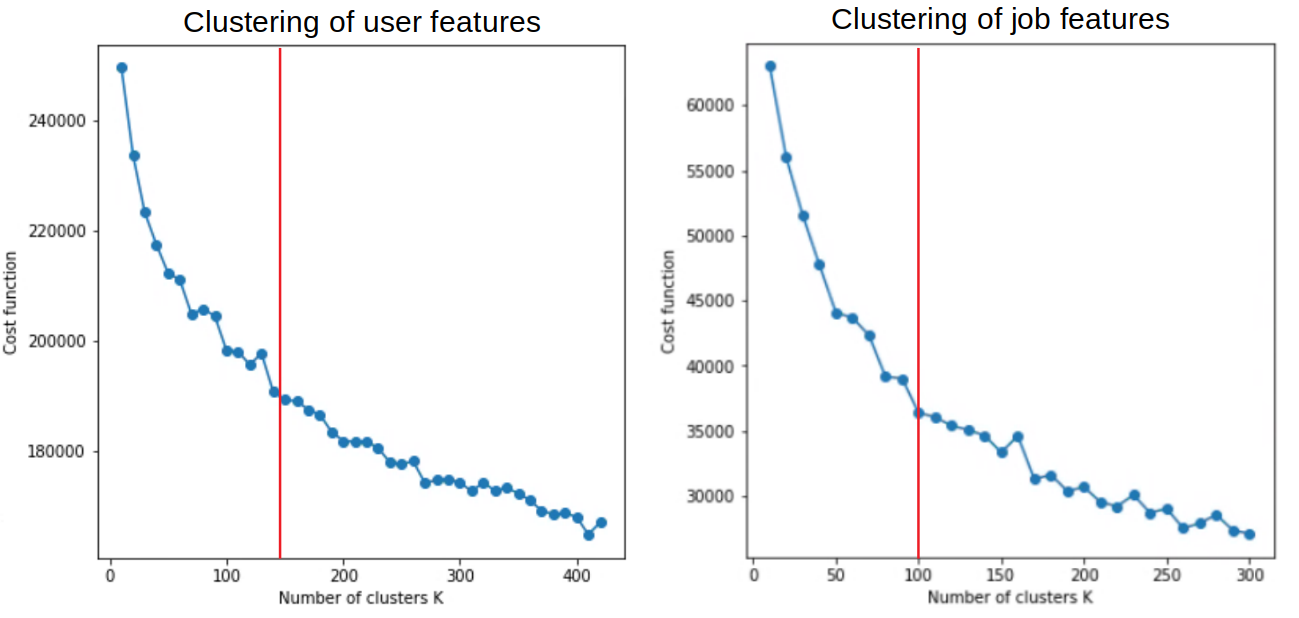
\includegraphics[width=\linewidth]{ThesisTemplate/Images/Clustering.png}
    \caption{\label{fig:eb} Elbow plots}
\end{figure}

% \begin{table}[h]
% \begin{footnotesize}
% \begin{tabular}{llll}
\toprule
\textbf{Scenario}   & \textbf{\# clusters}  & \textbf{Accuracy} & \textbf{MCC}    \\
\midrule
1                   & 225                   & 0.81              & 0.41            \\ %6.7
2                   & 275                   & 0.82              & 0.49            \\ %6.15
3                   & 300                   & 0.75              & 0.08            \\ %6.8
4                   & 100                   & 0.77              & 0.05            \\ %6.13
5                   & 225                   & 0.82              & 0.45            \\ %6.2
6                   & 300                   & 0.77              & 0.27            \\ %6.3
7                   & 250                   & 0.84              & 0.55            \\ %6.14 
9                   & 150                   & 0.79              & 0.27            \\ %6.12
10                  & 25                    & 0.15              & 0.11            \\ %6.4
11                  & 25                    & 0.93              & 0.92            \\ %6.6
12                  & 25                    & 0.11              & 0.05            \\ %6.10 
13                  & 25                    & 0.89              & 0.88            \\ %6.11
\bottomrule
\end{tabular}
% \end{footnotesize}
% \caption{\label{tab:clures} Best Results Clustering}
% \end{table}

\subsection{Results Content-Based Learning Models}
\mynote[author=Harrie]{Een confusion matrix zou hier heel goed werken, of anders iets van (percentage) false/true positives/negatives, omdate de MCC toch moeilijk te interpreteren is.}
When assessing the accuracy results it must be taken into account that the dataset exhibits a class imbalance of 79\% being positive labels and 21\% being negative labels. 
The consequence of this imbalance is that if the classifier predicts all labels to be positive it achieves 0.79 accuracy. 
This fallaciously suggests that the classification results are decent.
Here is where the utility of the Matthews correlation coefficient (MCC) comes into play, as the MCC in such case will be 0.00 because no labels are classified as negative. 

The classification results of the models are shown in table \ref{tab:res}.
For training and validation of all models a fixed split of 80/20 is used.
Judging only on the accuracy alone it does not seem to make a great difference which model is applied.
When the MCC scores are analyzed the Neural Network performs 10\% better than its closest rival and 52\% better than the baseline. 
The higher performance of MCC suggests better balanced predictions of both the positive and negative labels.
The best scores for the Neural Network were achieved with a setup of one hidden layer. 
When more hidden layers are added the performance decays gradually.
The more hidden layers the more complex patterns the Neural Network can learn, on the other hand this also increases the chance of overspecialization (overfitting) on the train data. 
Therefore, it can be argued that when extra layers are added the performance is worsens due to overfitting. 

\begin{table}[h]
\begin{footnotesize}
\begin{tabular}{lrr}
\toprule
\textbf{Model}      & \textbf{Accuracy} & \textbf{MCC}  \\
\midrule
Nearest Neighbors (baseline)   & 0.76              & 0.29          \\     
K-Nearest Neighbors & 0.80              & 0.35          \\
RandomForest        & 0.82              & 0.40          \\
Logistic Regression & 0.80              & 0.35          \\
Linear SVC          & 0.80              & 0.33          \\
Neural Network      & 0.81              & 0.44          \\
\bottomrule
\end{tabular}

\end{footnotesize}
\caption{\label{tab:res} Training Results Models}
\end{table}

\begin{table}[h]
\begin{footnotesize}
\begin{tabular}{l|l|l|r|r|}
    \multicolumn{3}{c}{\multirow{2}{*}}                          &  \multicolumn{2}{c}{\textbf{Actual labels}}   \\ 
    \cline{4-5}
    \multicolumn{3}{c|}{}                                        &Positive           &Negative                   \\
    \cline{3-5}
    \multicolumn{2}{l|}{\textbf{Predicted}}  &Positive           & 1,129      &111                  \\
    \cline{3-5}
    \multicolumn{2}{l|}{\textbf{labels}}     &Negative           & 190         &181                 \\
    \cline{3-5}
\end{tabular}





\end{footnotesize}
\caption{\label{tab:cmnn} Confusion Matrix Neural Network}
\end{table}

The MCC score is low and therefore also the precision, recall and F-measure were analyzed.
Overall the performance of all models is good on predicting the positive labels and bad when it comes to predict the negative labels.
Due to the class imbalance the classifiers display a tendency to overpredict the positive labels, and therefore it is hard to determine how well the positive labels are learned. 

\subsection{Ranking Results}
Another method to evaluate the classification of the positive labels is by ranking them and then retrieving the average rank.
To achieve that the train model predicts the label probability of each user-job combination, whereafter the average rank can be calculated.
There are 4,983 unique jobs (midpoint is 2,491), and the expectation would be that the positive labels would at least come in the top 100. 
The results show a different picture, for Logistic Regression the average rank of the positive labels is 2,611 and for the Neural Network 2,250.
The Neural Network performs best, but the results are not significant better than the random selection and definitely not close to an average rank below 100.



%logistic regression ranks the jobs for all users the same

%K-modes - descent, but no better learning results when predicting cluster or when added as extra feature
%hierarchical - good results on visual inspection, but no better learning results when predicting cluster or when added as extra feature (check this!)

% \todo{Content based Models}
% Neural network
    % One layer setup works best (assumption of overfitting when more layers are added)
% Logistic Regression
    % Ranking: same rankings for every user, because per row the user is the same and only the jobs are different
% Ranking
    % Random outcomes
    % validated by overfitting on subsample, predicted all 1

\todo{Strategies to improve}
% Under-oversampling worsen results
% Feature importance slight improvement of results

\section{Discussion}
\label{sec:disc}

% user features do not carry predictive power
%Ranking confirms that positive labels are not learned accurately

%introduction 
In this section the answering of the main research question (\ref{ssec:jrswb}) will be discussed, as well as the learnings (\ref{ssec:learnings}).

\subsection{A Job Recommender System for Welfare Beneficiaries}
\label{ssec:jrswb}

%Main Research Question
In this part we discuss the findings and answer the main Research Question~\ref{rq:mrq}: 
\begin{itemize}
	\item[] \em Can a content-based recommender system based on matching job openings to welfare beneficiaries be comparable to human customer managers?
\end{itemize}

%Discussion for answering the main research question
%How representative is the data?
\noindent The objective of this research was to study the feasibility of a Job Recommender System especially designed for welfare beneficiaries. 
The results presented in section \ref{sec:rslts} showed a challenge in recommending jobs with the available data.
This can in part be explained by the number of observations and the quality of them.
The provided dataset containing 8,265 observations was collected over a time period of five years in which ?????? persons in the municipality of Amsterdam received welfare benefits. %????? exacte aantal uitzoeken en aanvullen
Considering these figures the real number of occurred job matches is most likely to be in order of multitudes higher.
Therefore it can be questioned how representative the data is, because it is thought that it only represents  a small subset of the true number job matches that took place in that period.  
The small number of documented job matches can be attributed to a combination of factors.
First, not all welfare beneficiaries are obligated to apply for jobs.
Second, not all welfare beneficiaries have applied for jobs listed by the WSP.
Third and the most important factor is the lack of registration discipline by the customer managers.
According to domain experts there is a tendency to only register the most promising job matches.
This could also explain the observed overrepresentation of positive labels since a class imbalance towards the negative labels would rather be expected because it is assumed that people should apply for multiple jobs when they receive welfare benefits for a long period. 
Furthermore, when a job match gets documented in more than half of the cases (54\%) no feedback is received on the outcome.
Adding all these factors together it can be argued that the data is not representative for the total population of welfare beneficiaries within the city of Amsterdam. 

%cold-start problem and clustering
The cold start problem is an issue particular associated with Job Recommender Systems (JRS). In our case this problem is amplified by the preselection bias with 78\% of the observations being 1-to-1 relations (a user applies only once for a job, and for a job is applied only once). 
When analyzing the cold start problem it was found that it is plausible to segment the welfare beneficiaries in two general categories.
The first category consists of people who can easily find a job. 
It is expected that this group receives welfare benefits for a short time period and that they apply only once or just a couple of times for a job with mostly positive outcomes. 
The second category contains people for whom it is challenging to find a job. 
This group is expected to receive welfare benefits over a long period of time and therefore apply for a lot of jobs with predominantly negative results.
However, attempts to cluster the users in two or more clusters did not deliver promising results.
This could be likely explained by two reasons: 1) there are less or far more than two groups of users, or 2) only people from the first category are represented in the provided data. 
The second reason is interesting because it could explain that due to the preselection bias only people from the first category have made it into the dataset, and since this group commonly matches positively with job openings this causes the class imbalance.
If there are two groups of welfare beneficiaries the JRS should take that into consideration when learning to predict job matching outcomes, otherwise the JRS is optimized in predicting job matches for one group of users. 

%Why do the user features have no predictive power?
Another interesting finding presented in section~\ref{ssec:ir} is that job matches can be more accurately predicted when all user features are left out.  
A plausible explanation is that this is caused by how the user features are documented.
Before the data enters the JRS there are a couple of transfer/interpretation moments. 
The first is the verbal transfer from the welfare beneficiary to the customer manager.
The second takes place when the customer manager enters the information into the system.
The third is the extraction of the data from the system for the researcher of the JRS.
And finally the researcher applies feature engineering and other transformations before inputting the data into a machine learning model.
With every transfer errors and irregularities can arise, especially since at the transfer moments often assumptions need to be made that can possibly introduce bias.
It is thought that the first two transfer moments are most determining for the quality of the data, but they also introduce most of the bias and noise. The most probable cause is that there are various registration approaches between the different customer manager teams and also between the individual customers managers within the same team. 
Furthermore, over the years there have been changes appended in the documentation procedures, causing that fields in the system that had to be filled in a certain period were not filled  in another period.
Last and probably the most important factor is that a lot of the registered information is by nature highly subjective with many possible interpretations resulting in the main source of bias in the data. 
On the other hand it can also be imagined that the researcher of the JRS did introduce bias and error.
The preselection of features based on heuristics prior to the retrieval from the system/database is a moment that bias can have been imported into the data.
Moreover, during the feature engineering process also bias and error can have been entered into the data.
The finding that in our case the user features have no predictive power can presumably be attributed to a combination of the aforementioned factors.

%Temporal dependency 
Finally the data is assumed to exhibit a time dependency.
Hiring criteria change over time, and according to domain experts these should be updated at least every six months. 
During and in the aftermath of the financial crisis job hiring criteria became increasingly strict, but when the economy recovered and the labor market became tighter the hiring criteria started to lower. 
The thought is that this cycle affects welfare beneficiaries more than other job seekers because they are often at the lower end of the labor market.
This time-bound labor market dynamics can explain why the same types of jobs can have very different hiring criteria depending on the time they were posted.
This makes it harder for the machine learning models to identify and generalize patterns.
The solution would be to model the time dependency using a sliding window or another technique, however for this research this could not be applied because then the number of observations would get to low.  

%Summary/Conclusion
The disappointing results of the JRS can possibly also be contributed to the methods that were chosen or the features that were selected. 
However, it appears more likely that it can be attributed to the many challenges that reside in the data.
Therefore it can be argued that in our case it is currently not feasible to build a JRS with the available data in combination with the applied methods. 

%Answer to the Main Research Question
In conclusion to answer the main Research Question~\ref{rq:mrq}: it was found that for our study based on the available data its is unlikely that the outcomes of a content-based recommender system can match job openings with welfare beneficiaries in a comparable way as human customer managers. 
%Learnings
\subsection{Learnings}
\label{ssec:learnings}

%Quote
\textit{“…some machine learning projects succeed and some fail. What makes the difference?  Easily the most important factor is the features used.”} (Pedro Domingos, 2012) \nocite{domingos2012few} \\

\noindent In Data Science there is an emphasis on data, and consequently the quality of the available data determines more than other things the success of a Data Science research project.
In case of this research the provided data in the end turned out to be unsuitable to build a complex Job Recommender System (JRS). 

%Learnings
What can be learned from this? 
First of all that the availability of enough data with good quality is a prerequisite for researching the feasibility of a JRS.
What is enough data?
There is no absolute answer on that question. 
However, what is known is that other JRS systems have millions of observations at their disposal \cite{kenthapadi2017personalized, T.Al-Otaibi2012ASystems, Zheng2012JobSurvey, hong2013job}.
In our case the number of documented job matches was to low. 
This can be increased by a better registration discipline.
What is good quality data?
In general good data meets at least the following requirements: completeness, consistency, accuracy, time stamped, and complying with the industry standards. 
In our case the quality of the data lacked these characteristics: there are too many user features and to many options and fields to document user information, which also are inconsistently used. 

Secondly, the quality of the data was also negatively influenced by the fact that the choices concerning the data registration have been altered in certain periods of time.
Here also better registration is key.
The data quality could benefit from a simplified user profile and structured recording procedures. An additional advantage is that this will likely lower the administrative burden for the customer managers.

Third, the data process has various transfer moments where bias can come into the data. 
Excluding all bias is impossible, but can be limited by aligned procedures and proper data governance.

Overall the improvement of the quantity and quality of the data can be reached with appropriate data governance. 
This requires to think not only about the question “where do we need the data for now” but also “how do we organize our data in such a way that it also usable for future methods?”

%Conclusion
When data the prerequisites are met the implementation of JRS becomes feasible.
This will take time, maybe years, but is probably worth investment keeping in mind that proper data can be used for far more purposes than job recommendation alone.
When there enough quantity and quality of the data it is advised to redo this research. 


\section{Conclusion}
\label{sec:concl}

%introduction
A Job Recommender System (JRS) is a complex system with many facets, implementing one is not a straightforward procedure.
In the Results chapter (\ref{sec:rslts}) it is shown that the methods that were tested during this research did not result in a working JRS.
In the section Discussion (\ref{sec:disc}) it is argued that this outcome can be attributed to the quantity and quality of the data, rather than the machine learning models that were applied.
It is believed that a JRS is still possible, however not with the data that was available for this research project.

%Conclusion
In conclusion it is unlikely that a JRS based on the tested methods in combination with the available data can be comparable to human customer managers.
However, when in the future the data quantity and quality is improved a JRS might become feasible.




% Data quality and sample size restrict results
% It can be done things need to be improved
% Nearest neighbor recommender could be implemented
% Sliding window for capturing temporal dynamics (x months sliding a month)
% validity, generalizability, scalability

\section{Future Work}
\label{sec:fut}

%Introduction
It is advised to do several researches and to take measures prior to a new feasibility study of a Job Recommender System (JRS).
The most important ones are described briefly in this section.

%prerequisites
Measures can be taken to improve the registration of job matches outcomes.
Measures can be taken to reduce the bias and noise in the data processing.
Here standardized procedures and user profiles can be researched and implemented.
This kind of preliminary research would be more in the field of Business Economics, Lean Six Sigma and/or Operational Excellence than in the field of Data Science (alone).
In anticipation of that an in depth social research is advised to determine which user attributes are the most important for finding a job.
Finally, it can be researched if jobs can be grouped in such a way that similar jobs have similar hiring criteria.

%follow-up studies
When the quantity and quality of data is improved a new JRS feasibility study can be done.
It is advised to split this study into two phases (or even in two  projects) with multiple Data Science researchers because there are many facets to a JRS. 
Moreover it is very well possible that when the new data are available there might be different JRS solutions that can be investigated.
Therefore the first phase should emphasize on researching the most promising methods for a JRS based on the new data.
The second phase is to conduct a user study to validate the most promising methods for the JRS in a real life setting.
It can be imagined that such an approach could be a collaboration between a Data Scientist and a Social and/or Economic researcher.  

%conclusion
Building a JRS is quite comprehensive, to do it properly requires multiple extensive research phases or projects preceding that.


\section*{Acknowledgements}
I would like to thank the municipality of Amsterdam for offering me the opportunity to do this research project. 
The municipality me the trust and the freedom to carry out this project.
It was a pleasure to work in such a friendly and encouraging environment.
I would like to thank Camiel de Wit, Erik-Jan Hombergen and Jovita Bos for providing whatever data I needed, and for always willing to help and to answer my questions. 
Also I would like to thank Toetske Renier for getting me on board in the project team and helping me to break down any barriers. 
I would like to specially thank Lonneke van Oirschot for her guidance as my supervisor within the municipality of Amsterdam, without her effort and expertise this project would not have been possible. 
Last but not least I would like to thank Harrie Oosterhuis for his role as my supervisor. 
His expert knowledge and willingness to help really contributed to completing this thesis project.

% References
\bibliographystyle{plain}
\bibliography{9_references}

%APPENDIX
\pagebreak
\onecolumn
\appendix

\section{Appendix}

\subsection{Used Hyperparameters}
\label{ssec:ushp}
\begin{table}[h]
\begin{footnotesize}
\begin{tabular}{lll}
    \toprule
    \textbf{Algorithm}                  & \textbf{Scikit-learn}     & \textbf{Hyperparameters}  \\
    \midrule
    Nearest Neighbors                   & NearestNeighbors()        & n\_neighbors = 2          \\
                                        &                           & algorithm = “brute”       \\
    \midrule
    K-Nearest Neighbors                 & KNeighborsClassifier()    & n\_neighbors = 8          \\
    \midrule
    RandomForest                        & RandomForest()            & n\_estimators = 231       \\
                                        &                           & min\_samples\_split = 2   \\
                                        &                           & min\_samples\_leaf = 1    \\
                                        &                           & max\_features = “sqrt”    \\
                                        &                           & max\_depth = None         \\
                                        &                           & bootstrap = False         \\
                                        &                           & random\_state = 7         \\
    \midrule
    Logistic Regression                 & LogisticRegression()      & random\_state = 0         \\
                                        &                           & solver = “sag”            \\
                                        &                           & multi\_class = “ovr”      \\
                                        &                           & max\_iter = 10000         \\
    \midrule
    Linear Support Vector Classification& LinearSVC()               & random\_state = 7         \\
    \midrule
    Neural Network                      & MLPClassifier()           & activation = ‘relu’       \\
                                        &                           & hidden\_layers\_sizes = dataset length    \\
                                        &                           & learning\_rate = “constant”   \\
                                        &                           & max\_iter = 10000         \\
                                        &                           & n\_iter\_no\_change = 10  \\
                                        &                           & random\_state = 7         \\
                                        &                           & solver = “adam”           \\
                                        &                           & early\_stopping = “False” \\
    \bottomrule
\end{tabular}



\end{footnotesize}
\caption{\label{tab:Hyperparameters} Used Hyperparameters}
\end{table}

\subsection{K-Nearest Neighbors: Finding the Optimum Number of Neighbors}
\label{ssec:fonn}
\begin{figure}[h]
    \centering
    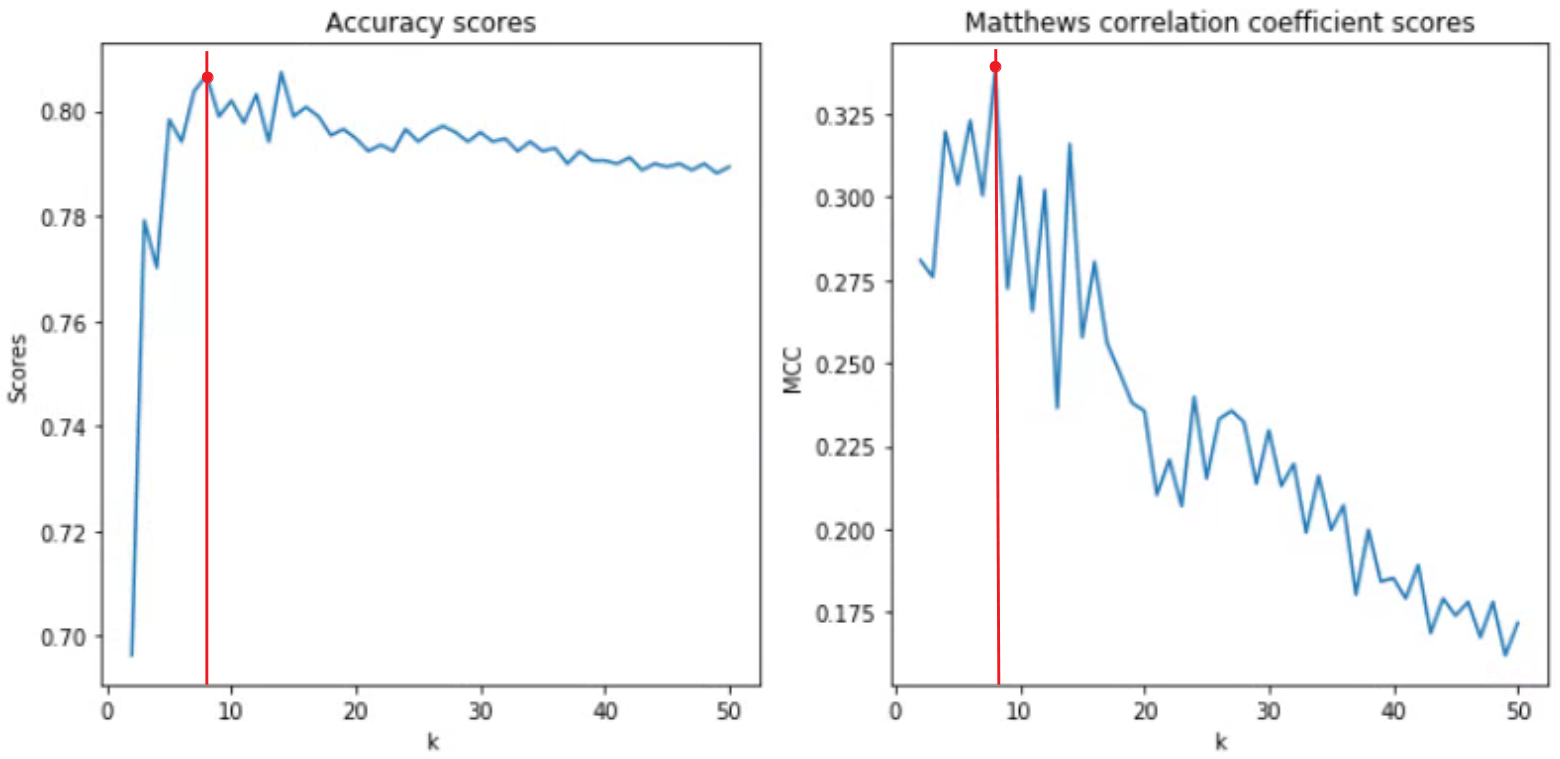
\includegraphics[width=.7\linewidth]{ThesisTemplate/Images/KNN_n_neighbors.png}
    \caption{K-Nearest Neighbors: Finding the Optimum Number of Neighbors}
\end{figure}

\subsection{Neural Network: Results K-Modes Clustering}
\label{ssec:cluscen}
\begin{table}[H]
\begin{footnotesize}
\begin{tabular}{llllll}
\toprule
\textbf{Scenario}   & \textbf{Features (\textit{X})}    & \textbf{Labels (\textit{y})}  & \textbf{Clusters} & \textbf{Accuracy} & \textbf{MCC}        \\
\midrule
baseline            & users + jobs                      & labels                        & -                     & 0.81              & 0.44            \\
baseline            & users                             & labels                        & -                     & 0.71              & 0.03            \\
baseline            & jobs                              & labels                        & -                     & 0.84              & 0.53            \\
\midrule
1                   & users + jobs + user clusters      & labels                        & 225                   & 0.81              & 0.41            \\ %6.7
2                   & jobs + user clusters              & labels                        & 275                   & 0.82              & 0.49            \\ %6.15
3                   & users + user clusters             & labels                        & 300                   & 0.75              & 0.08            \\ %6.8
4                   & user clusters                     & labels                        & 100                   & 0.77              & 0.05            \\ %6.13
5                   & users + jobs + job clusters       & labels                        & 225                   & 0.82              & 0.45            \\ %6.2
6                   & users + job clusters              & labels                        & 300                   & 0.77              & 0.27            \\ %6.3
7                   & jobs + job clusters               & labels                        & 250                   & 0.84              & 0.55            \\ %6.14
8                   & job clusters                      & labels                        & 150                   & 0.79              & 0.27            \\ %6.12
9                   & users                             & job clusters                  & 25                    & 0.15              & 0.11            \\ %6.4
10                  & users + jobs                      & job clusters                  & 25                    & 0.93              & 0.92*            \\ %6.6
12                  & jobs                              & user clusters                 & 25                    & 0.11              & 0.05            \\ %6.10 
13                  & users + jobs                      & user clusters                 & 25                    & 0.89              & 0.88*            \\ %6.11
\bottomrule
\tiny{*Overfitting} \\
\end{tabular}

\end{footnotesize}
\caption{\label{tab:clusc} Neural Network: K-Modes Clustering Scenarios \& Results}
\end{table}

\subsection{K-Means: Finding the Optimum Number of Clusters}
\label{ssec:Kmeans}
\begin{figure}[h]
    \centering
    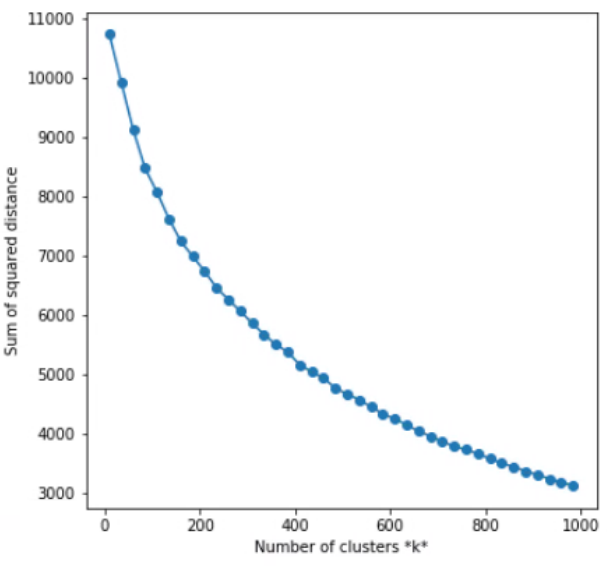
\includegraphics[width=.4\linewidth]{ThesisTemplate/Images/K-means.png}
    \caption{K-Means: Elbow Plot NLP Clustering}
\end{figure}

\subsection{Neural Network: Hierarchical Clustering Scenarios}
\label{ssec:hieclu}
\begin{table}[H]
\begin{footnotesize}
\begin{tabular}{lllll}
\toprule
\textbf{Scenario}   & \textbf{Features (\textit{X})}    & \textbf{Labels (\textit{y})}  & \textbf{Accuracy} & \textbf{MCC}        \\
\midrule
baseline            & users + jobs                      & labels                        & 0.81              & 0.44            \\
baseline            & jobs                              & labels                        & 0.84              & 0.53            \\
\midrule
1                   & users + jobs + job clusters       & labels                        & 0.81              & 0.41            \\ %6.2
2                   & users + job clusters              & labels                        & 0.74              & 0.10            \\ %6.3
3                   & jobs + job clusters               & labels                        & 0.83              & 0.48            \\ %6.14
4                   & users                             & job clusters                  & 0.25              & 0.04            \\ %6.4
5                   & users + jobs                      & job clusters                  & 0.71              & 0.66            \\ %6.6
\bottomrule
\end{tabular}

\end{footnotesize}
\caption{\label{tab:hieclu} Neural Network: Hierarchical Clustering Scenarios \& Results}
\end{table}

\subsection{Confusion Matrices}
\label{ssec:cm}
\begin{table}[H]
\begin{footnotesize}
\begin{tabular}{llrr}
    \toprule
    \textbf{Algorithm}                  &                           &                           &                           \\
    \midrule
    Nearest Neighbors                   &                           & Positive Labels           & Negative Labels            \\
                                        & Positive Labels           & 5,482                     & 1,008                      \\
                                        & Negative Labels           & 982                       & 793                        \\
    \midrule
    K-Nearest Neighbors                 &                           & Positive Labels           & Negative Labels            \\
                                        & Positive Labels           & 1,184                     & 56                         \\
                                        & Negative Labels           & 259                       & 112                        \\
    \midrule
    RandomForest                        &                           & Positive Labels           & Negative Labels            \\
                                        & Positive Labels           & 1,203                     & 37                         \\
                                        & Negative Labels           & 256                       & 115                        \\
    \midrule
    Logistic Regression                 &                           & Positive Labels           & Negative Labels            \\
                                        & Positive Labels           & 1,155                     & 85                         \\
                                        & Negative Labels           & 241                       & 130                        \\
    \midrule
    Linear Support Vector Classification&                           & Positive Labels           & Negative Labels           \\
                                        & Positive Labels           & 1,158                     & 82                        \\
                                        & Negative Labels           & 249                       & 122                       \\
    \midrule
    Neural Network                      &                           & Positive Labels           & Negative Labels           \\
                                        & Positive Labels           & 1,129                     & 111                       \\
                                        & Negative Labels           & 190                       & 181                       \\
    \midrule
    \textit{Legend}                     &                           & Positive Labels           & Negative Labels            \\
                                        & Positive Labels           & \textit{True positives}   & \textit{False negatives}   \\
                                        & Negative Labels           & \textit{False positives}  & \textit{True Negatives}    \\
    \bottomrule
\end{tabular}
\end{footnotesize}
\caption{\label{tab:cm} Confusion Matrices}
\end{table}

\subsection{Results Undersampling and Oversampling}
\label{ssec:ruo}
\begin{table}[H]
\begin{footnotesize}
\begin{tabular}{l|ll|ll|ll}
& \multicolumn{2}{c|}{\textbf{Baseline}} & \multicolumn{2}{c|}{\textbf{Undersampling}}  & \multicolumn{2}{c}{\textbf{Oversampling}} \\
\toprule
\textbf{Algorithm}      & Accuracy  & MCC   & Accuracy  & MCC   & Accuracy  & MCC   \\
\midrule                       
Nearest Neighbors       & 0.76      & 0.29  & 0.69      & 0.36  & 0.78      & 0.58  \\
K-Nearest Neighbors     & 0.80      & 0.35  & 0.69      & 0.35  & 0.37      & 0.16  \\
RandomForest            & 0.82      & 0.40  & 0.78      & 0.51  & 0.80      & 0.34  \\
Logistic Regression     & 0.80      & 0.35  & 0.72      & 0.38  & 0.79      & 0.34  \\
Linear SVC              & 0.80      & 0.35  & 0.72      & 0.37  & 0.78      & 0.32  \\
Neural Network          & 0.81      & 0.44  & 0.73      & 0.40  & 0.80      & 0.39  \\
\bottomrule
\end{tabular}
\end{footnotesize}
\caption{\label{tab:ruo} Results Undersampling and Oversampling}
\end{table}

\subsection{Results Feature Importance Methods}
\label{ssec:fi}
\begin{table}[H]
\begin{footnotesize}
\begin{tabular}{l|ll|ll|ll|ll}
& \multicolumn{2}{c|}{\textbf{Baseline}} & \multicolumn{2}{c|}{\textbf{Chi-Square Test}}  & \multicolumn{2}{c|}{\textbf{BFE}} & \multicolumn{2}{c}{\textbf{RFECV}} \\
\toprule
\textit{\# Features}& \multicolumn{2}{c|}{\textit{438}} & \multicolumn{2}{c|}{\textit{180}}  & \multicolumn{2}{c|}{\textit{116}} & \multicolumn{2}{c}{\textit{115}} \\
\midrule
\textbf{Algorithm}      & Accuracy  & MCC   & Accuracy  & MCC   & Accuracy  & MCC   & Accuracy  & MCC \\
\midrule                       
Nearest Neighbors       & 0.76      & 0.29  & 0.78      & 0.33  & 0.81      & 0.46  & 0.81      & 0.46 \\
K-Nearest Neighbors     & 0.80      & 0.35  & 0.80      & 0.34  & 0.81      & 0.41  & 0.81      & 0.38 \\
RandomForest            & 0.82      & 0.40  & 0.81      & 0.37  & 0.84      & 0.50  & 0.83      & 0.50 \\
Logistic Regression     & 0.80      & 0.35  & 0.80      & 0.37  & 0.81      & 0.36  & 0.81      & 0.38 \\
Linear SVC              & 0.80      & 0.35  & 0.81      & 0.37  & 0.80      & 0.35  & 0.80      & 0.36 \\
Neural Network          & 0.81      & 0.44  & 0.80      & 0.38  & 0.81      & 0.43  & 0.83      & 0.46 \\
\bottomrule
\multicolumn{9}{l}{\tiny{BFE: Backwards Feature Elimination, RFECV: Recursive Feature Elimination with Cross-Validation}}
\end{tabular}


\end{footnotesize}
\caption{\label{tab:fi} Results Feature Importance Methods}
\end{table}






 
\end{document}
